\documentclass[conference,letterpaper]{IEEEtran}
\IEEEoverridecommandlockouts
\usepackage{cite}
\usepackage{amsmath,amssymb}
\usepackage{graphicx}
\usepackage{booktabs}
\usepackage{xcolor}
\usepackage{fancyvrb}
\usepackage{tikz}
\usetikzlibrary{arrows.meta,positioning}
\usepackage{fancyhdr}
\usepackage{xurl}
\usepackage[hidelinks]{hyperref}
% generated by paper_gtdla/make_macros.py; do not edit
\newcommand{\aidLeadH}{24}
\newcommand{\aidShare}{0.5}
\newcommand{\anchorMax}{5.9}
\newcommand{\anchorMin}{1.6}
\newcommand{\anchorRatio}{4.0}
\newcommand{\autoHiMin}{60}
\newcommand{\autoLoMin}{15}
\newcommand{\autoMax}{31}
\newcommand{\autoMin}{9}
\newcommand{\chErrInNE}{2}
\newcommand{\chErrInPA}{2}
\newcommand{\chErrOutNE}{34}
\newcommand{\chErrOutPA}{29}
\newcommand{\chNE}{281}
\newcommand{\chPooledInNE}{1.01}
\newcommand{\chPooledInPA}{1.00}
\newcommand{\chPooledOutNE}{0.92}
\newcommand{\chPooledOutPA}{0.79}
\newcommand{\chRatioInNE}{0.99}
\newcommand{\chRatioInPA}{1.00}
\newcommand{\chRatioOutNE}{1.06}
\newcommand{\chRatioOutPA}{0.93}
\newcommand{\chWithinInNE}{100}
\newcommand{\chWithinInPA}{100}
\newcommand{\chWithinOutNE}{41}
\newcommand{\chWithinOutPA}{43}
\newcommand{\crewsFiveOverSeventyTwo}{$-$47}
\newcommand{\crewsFiveOverSeventyTwoAbs}{47}
\newcommand{\crewsFivePaid}{+14}
\newcommand{\crewsFivePaidAbs}{14}
\newcommand{\crewsFiveSaidi}{$-$11}
\newcommand{\crewsFiveSaidiAbs}{11}
\newcommand{\crewsFiveTravel}{+22}
\newcommand{\crewsFiveTravelAbs}{22}
\newcommand{\crewsMaxOverSeventyTwo}{$-$70}
\newcommand{\crewsMaxOverSeventyTwoAbs}{70}
\newcommand{\crewsMaxPaid}{+28}
\newcommand{\crewsMaxPaidAbs}{28}
\newcommand{\crewsMaxSaidi}{$-$19}
\newcommand{\crewsMaxSaidiAbs}{19}
\newcommand{\crewsMaxTravel}{+35}
\newcommand{\crewsMaxTravelAbs}{35}
\newcommand{\crewsMinOverSeventyTwo}{+355}
\newcommand{\crewsMinOverSeventyTwoAbs}{355}
\newcommand{\crewsMinPaid}{$-$33}
\newcommand{\crewsMinPaidAbs}{33}
\newcommand{\crewsMinSaidi}{+89}
\newcommand{\crewsMinSaidiAbs}{89}
\newcommand{\crewsMinTravel}{$-$53}
\newcommand{\crewsMinTravelAbs}{53}
\newcommand{\crewsThreeOverSeventyTwo}{+82}
\newcommand{\crewsThreeOverSeventyTwoAbs}{82}
\newcommand{\crewsThreePaid}{$-$14}
\newcommand{\crewsThreePaidAbs}{14}
\newcommand{\crewsThreeSaidi}{+20}
\newcommand{\crewsThreeSaidiAbs}{20}
\newcommand{\crewsThreeTravel}{$-$25}
\newcommand{\crewsThreeTravelAbs}{25}
\newcommand{\crewsTwoOverSeventyTwo}{+234}
\newcommand{\crewsTwoOverSeventyTwoAbs}{234}
\newcommand{\crewsTwoPaid}{$-$28}
\newcommand{\crewsTwoPaidAbs}{28}
\newcommand{\crewsTwoSaidi}{+59}
\newcommand{\crewsTwoSaidiAbs}{59}
\newcommand{\crewsTwoTravel}{$-$45}
\newcommand{\crewsTwoTravelAbs}{45}
\newcommand{\custMNE}{7.4}
\newcommand{\custMPA}{7.2}
\newcommand{\custPerJob}{35}
\newcommand{\decisionH}{6}
\newcommand{\fleetNE}{342}
\newcommand{\fleetPA}{302}
\newcommand{\guardH}{48}
\newcommand{\gustCaidiFive}{11.7}
\newcommand{\gustCaidiZero}{8.8}
\newcommand{\gustEndFive}{148}
\newcommand{\gustEndZero}{121}
\newcommand{\gustInterX}{2.0}
\newcommand{\gustOverNinetySixX}{13.0}
\newcommand{\gustOverSeventyTwoX}{7.2}
\newcommand{\gustPaidCH}{+50}
\newcommand{\gustPaidCHAbs}{50}
\newcommand{\gustSaidiMinusFiveX}{0.39}
\newcommand{\gustSaidiX}{3.3}
\newcommand{\interNE}{15.4}
\newcommand{\isaiasAfterPeak}{24}
\newcommand{\isaiasAidAfterPeak}{17}
\newcommand{\isaiasCHObsCT}{33.3}
\newcommand{\isaiasCHObsRest}{2.1}
\newcommand{\isaiasCHSimCT}{22.0}
\newcommand{\isaiasCHSimRest}{5.7}
\newcommand{\isaiasDamageNinety}{17}
\newcommand{\isaiasOutNinetySix}{201}
\newcommand{\isaiasOutSeventyTwo}{358}
\newcommand{\isaiasOutTwentyFour}{787}
\newcommand{\isaiasPeak}{1,220}
\newcommand{\isaiasSaidiObs}{552}
\newcommand{\lagFortyEightOverNinetySix}{+44}
\newcommand{\lagFortyEightOverNinetySixAbs}{44}
\newcommand{\lagFortyEightSaidi}{+8}
\newcommand{\lagFortyEightSaidiAbs}{8}
\newcommand{\lagSeventyTwoOverNinetySix}{+105}
\newcommand{\lagSeventyTwoOverNinetySixAbs}{105}
\newcommand{\lagSeventyTwoSaidi}{+12}
\newcommand{\lagSeventyTwoSaidiAbs}{12}
\newcommand{\lagTwelveOverNinetySix}{$-$16}
\newcommand{\lagTwelveOverNinetySixAbs}{16}
\newcommand{\lagTwelveSaidi}{$-$7}
\newcommand{\lagTwelveSaidiAbs}{7}
\newcommand{\nAnchors}{five}
\newcommand{\nCounties}{189}
\newcommand{\nCountiesNE}{67}
\newcommand{\nCountiesPA}{122}
\newcommand{\nRunsDemo}{4,212}
\newcommand{\nSeeds}{3}
\newcommand{\nStorms}{85}
\newcommand{\nStormsNE}{39}
\newcommand{\nStormsPA}{46}
\newcommand{\nTests}{55}
\newcommand{\nValInNE}{39}
\newcommand{\nValInPA}{46}
\newcommand{\nValOutNE}{39}
\newcommand{\nValOutPA}{46}
\newcommand{\overNinetySixNE}{167}
\newcommand{\overSeventyTwoNE}{467}
\newcommand{\overTwentyFourNE}{4.0}
\newcommand{\peakAllMax}{0.94}
\newcommand{\peakAllMin}{0.88}
\newcommand{\peakRatioInNE}{0.91}
\newcommand{\peakRatioInPA}{0.94}
\newcommand{\peakRatioOutNE}{0.89}
\newcommand{\peakRatioOutPA}{0.93}
\newcommand{\pjHigh}{55}
\newcommand{\pjHighBusy}{2.83}
\newcommand{\pjHighFleet}{+17}
\newcommand{\pjHighFleetAbs}{17}
\newcommand{\pjHighGust}{3.10}
\newcommand{\pjHighLag}{+7}
\newcommand{\pjHighLagAbs}{7}
\newcommand{\pjHighOverNinetySix}{103}
\newcommand{\pjHighRepair}{3.9}
\newcommand{\pjHighSaidi}{2,262}
\newcommand{\pjLow}{20}
\newcommand{\pjLowBusy}{4.20}
\newcommand{\pjLowFleet}{+23}
\newcommand{\pjLowFleetAbs}{23}
\newcommand{\pjLowGust}{3.51}
\newcommand{\pjLowLag}{+9}
\newcommand{\pjLowLagAbs}{9}
\newcommand{\pjLowOverNinetySix}{249}
\newcommand{\pjLowRepair}{2.0}
\newcommand{\pjLowSaidi}{2,268}
\newcommand{\pjMid}{35}
\newcommand{\pjMidBusy}{3.43}
\newcommand{\pjMidFleet}{+20}
\newcommand{\pjMidFleetAbs}{20}
\newcommand{\pjMidGust}{3.31}
\newcommand{\pjMidLag}{+8}
\newcommand{\pjMidLagAbs}{8}
\newcommand{\pjMidOverNinetySix}{167}
\newcommand{\pjMidRepair}{2.8}
\newcommand{\pjMidSaidi}{2,268}
\newcommand{\repairCV}{0.6}
\newcommand{\repairMax}{20}
\newcommand{\repairMed}{2.5}
\newcommand{\ruGuaOverNinetySix}{273}
\newcommand{\ruGuaOverSeventyTwo}{677}
\newcommand{\ruGuaOverTwentyFour}{4.16}
\newcommand{\ruGuaSaidi}{2,398}
\newcommand{\ruGuaSaidiRel}{+5.7}
\newcommand{\ruGuaSaidiRelAbs}{5.7}
\newcommand{\ruGuaTravel}{339}
\newcommand{\ruGuaTravelRel}{$-$0.2}
\newcommand{\ruGuaTravelRelAbs}{0.2}
\newcommand{\ruGuaWorst}{24.3}
\newcommand{\ruGuaWorstRel}{+6}
\newcommand{\ruGuaWorstRelAbs}{6}
\newcommand{\ruLarOverNinetySix}{167}
\newcommand{\ruLarOverSeventyTwo}{467}
\newcommand{\ruLarOverTwentyFour}{4.02}
\newcommand{\ruLarSaidi}{2,268}
\newcommand{\ruLarSaidiRel}{+0.0}
\newcommand{\ruLarSaidiRelAbs}{0.0}
\newcommand{\ruLarTravel}{340}
\newcommand{\ruLarTravelRel}{+0.0}
\newcommand{\ruLarTravelRelAbs}{0.0}
\newcommand{\ruLarWorst}{23.0}
\newcommand{\ruLarWorstRel}{+0}
\newcommand{\ruLarWorstRelAbs}{0}
\newcommand{\ruOldOverNinetySix}{944}
\newcommand{\ruOldOverSeventyTwo}{2,161}
\newcommand{\ruOldOverTwentyFour}{8.09}
\newcommand{\ruOldSaidi}{4,310}
\newcommand{\ruOldSaidiRel}{+90.0}
\newcommand{\ruOldSaidiRelAbs}{90.0}
\newcommand{\ruOldTravel}{251}
\newcommand{\ruOldTravelRel}{$-$26.2}
\newcommand{\ruOldTravelRelAbs}{26.2}
\newcommand{\ruOldWorst}{40.2}
\newcommand{\ruOldWorstRel}{+74}
\newcommand{\ruOldWorstRelAbs}{74}
\newcommand{\ruProOverNinetySix}{168}
\newcommand{\ruProOverSeventyTwo}{468}
\newcommand{\ruProOverTwentyFour}{3.99}
\newcommand{\ruProSaidi}{2,258}
\newcommand{\ruProSaidiRel}{$-$0.5}
\newcommand{\ruProSaidiRelAbs}{0.5}
\newcommand{\ruProTravel}{330}
\newcommand{\ruProTravelRel}{$-$3.1}
\newcommand{\ruProTravelRelAbs}{3.1}
\newcommand{\ruProWorst}{18.0}
\newcommand{\ruProWorstRel}{$-$22}
\newcommand{\ruProWorstRelAbs}{22}
\newcommand{\saidiNE}{2,268}
\newcommand{\setupH}{0.5}
\newcommand{\speedKmh}{60}
\newcommand{\tFiftyInNE}{2}
\newcommand{\tFiftyInPA}{2}
\newcommand{\tFiftyOutNE}{5}
\newcommand{\tFiftyOutPA}{5}
\newcommand{\tNinetyInNE}{2}
\newcommand{\tNinetyInPA}{6}
\newcommand{\tNinetyOutNE}{3}
\newcommand{\tNinetyOutPA}{7}
\newcommand{\trigHighSaidi}{+0.9}
\newcommand{\trigHighSaidiAbs}{0.9}
\newcommand{\trigLowSaidi}{$-$0.7}
\newcommand{\trigLowSaidiAbs}{0.7}
\newcommand{\triggerPct}{1}
\newcommand{\version}{0.3.0}


% Running header of the conference on every page, copyright line at the foot of the first page
\fancypagestyle{gtd}{\fancyhf{}\fancyhead[C]{\small\itshape PES GT\&D Latin America 2027}%
  \renewcommand{\headrulewidth}{0pt}\renewcommand{\footrulewidth}{0pt}}
\fancypagestyle{gtdfirst}{\fancyhf{}\fancyhead[C]{\small\itshape PES GT\&D Latin America 2027}%
  \fancyfoot[C]{\footnotesize \textcopyright 2027 IEEE}%
  \renewcommand{\headrulewidth}{0pt}\renewcommand{\footrulewidth}{0pt}}
\setlength{\headheight}{12pt}
\pagestyle{gtd}

% Table captions on one line, as in the conference template: "TABLE I. Caption" in small caps
\makeatletter
\long\def\@makecaption#1#2{%
  \ifx\@captype\@IEEEtablestring
    \begin{center}\footnotesize\textsc{#1. #2}\end{center}\vspace{-4pt}%
  \else
    \vskip 0.3\baselineskip
    \setbox\@tempboxa\hbox{\footnotesize #1.~#2}%
    \ifdim \wd\@tempboxa >\hsize \footnotesize #1.~#2\par
    \else \hbox to\hsize{\hfil\box\@tempboxa\hfil}\fi
  \fi}
\def\tablename{Table}
\makeatother
\renewcommand{\IEEEkeywordsname}{Keywords}

% Four authors in two rows of two
\makeatletter
\newcommand{\linebreakand}{\end{@IEEEauthorhalign}\hfill\mbox{}\par\mbox{}\hfill\begin{@IEEEauthorhalign}}
\makeatother

\begin{document}

\title{StormCrews: An Open Simulator of Distribution\\Restoration After Storms}

\author{%
\IEEEauthorblockN{Abraham Jes\'us Boh\'orquez G\'omez}
\IEEEauthorblockA{\textit{Department of Industrial Engineering}\\
\textit{Universidad de los Andes}\\
Bogot\'a, Colombia\\
a.bohorquezg@uniandes.edu.co}
\and
\IEEEauthorblockN{Juan Jos\'e Murillo Aristiz\'abal}
\IEEEauthorblockA{\textit{Department of Industrial Engineering}\\
\textit{Universidad de los Andes}\\
Bogot\'a, Colombia\\
j.murilloa@uniandes.edu.co}
\linebreakand
\IEEEauthorblockN{Alejandra Tabares Pozos}
\IEEEauthorblockA{\textit{Department of Industrial Engineering}\\
\textit{Universidad de los Andes}\\
Bogot\'a, Colombia\\
a.tabaresp@uniandes.edu.co}
\and
\IEEEauthorblockN{Pablo Jos\'e Cort\'es Sanabria}
\IEEEauthorblockA{\textit{Department of Industrial Engineering}\\
\textit{Universidad de los Andes}\\
Bogot\'a, Colombia\\
pj.cortes716@uniandes.edu.co}}

\maketitle
\thispagestyle{gtdfirst}
\setcounter{dbltopnumber}{2}

\begin{abstract}
After a storm, how long customers stay without power depends on decisions a utility controls: how many crews it has,
where it sends them, which repairs go first and when it asks neighboring utilities for help. StormCrews is an
open-source Python simulator of those decisions. It replays \nStorms{} real storms of 2018 to 2025 in \nCounties{}
counties of New England, Pennsylvania and West Virginia, built only from public data, and reports each run in
reliability terms: the storm's contribution to SAIDI, customers out beyond 24, 72 and 96 hours, crew-hours and crews on
duty. Damage arrives hour by hour as in the outage records, crews travel and repair jobs, and mutual aid joins after a
lag. A restoration rule takes a few lines of code and runs on every storm with common random numbers, and a fitted
damage model changes the weather of a real storm. Calibrated per storm, with the fleet set from crew counts that
utilities reported in public filings, the simulator reproduces observed customer-hours. With its repair parameters
predicted from the other storms instead, a single storm's customer-hours miss by \chErrOutNE\,\% at the median in New
England. The inputs, the decisions and the outputs are described, the valid uses are stated, and a weather
what-if, a sweep of crews and mutual-aid lag and a comparison of restoration rules illustrate the tool.
\end{abstract}

\begin{IEEEkeywords}
\itshape distribution system restoration, reliability indices, resilience, repair crews, mutual assistance,
discrete-event simulation, open-source software
\end{IEEEkeywords}

\section{Introduction}

Severe weather causes the largest outages on distribution grids, and restoring service afterwards is an operations
problem with planning consequences \cite{wang2016review,panteli2015grid}. Damage keeps appearing for hours after the
first outages. The control room sees customers out by area, not the faults behind them. Repairs take uncertain times,
crews lose hours driving, and crews borrowed from other utilities arrive hours or days after the request. A planner
who wants to know how much a larger local fleet, a faster mutual-aid agreement or a different dispatch rule would
change the reliability indices of a bad season has few tools to ask with.

Fig.~\ref{fig:problem} shows the problem on a real storm. When Tropical Storm Isaias crossed New England in August
2020, customers out peaked at \isaiasPeak{} thousand, yet \isaiasAfterPeak\,\% of the customers who lost power did so
after that hour, and nine tenths of the damage had arrived only \isaiasDamageNinety{} hours after the peak. A day
after the peak \isaiasOutTwentyFour{} thousand customers were still out, and four days after it \isaiasOutNinetySix{}
thousand. The event added \isaiasSaidiObs{} minutes to the region's SAIDI, counting major event days.

\begin{figure}[t]
\centering
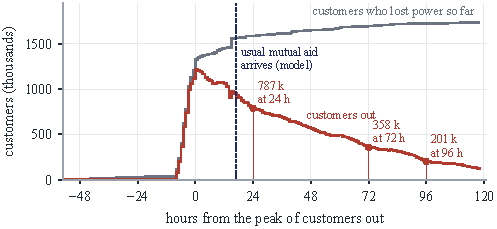
\includegraphics[width=\columnwidth]{figures/problem.pdf}
\caption{Damage keeps arriving after the peak and restoration takes days. Tropical Storm Isaias in New England, August
2020: customers out (red) and customers who had lost power so far (gray), EAGLE-I hourly records, with customers still
out 24, 72 and 96 hours after the peak. The dashed line marks when the usual mutual aid, requested once \triggerPct\,\% of
customers are out, joins in the simulator.}
\label{fig:problem}
\end{figure}

The usual tools answer other questions. Network optimization schedules repairs and switching on a known feeder model
\cite{arif2018outage}. Agent-based and statistical models of restoration time are fitted on one utility's private records
\cite{wanik2018etr,walsh2018abm}, so others cannot rerun them. StormCrews sits between the two. It needs no
network model, only the customers out in each area hour by hour, and it is calibrated and checked against real storms
from public records, so anyone can rerun every number.

The contribution is the tool itself, an open and tested simulator of crews, mutual aid and restoration rules on
\nStorms{} real storms whose outputs are the reliability quantities planners and regulators already track.

\section{What StormCrews Does}\label{sec:what}

\subsection{Inputs}

For each storm the engine needs the customers newly out in each area $k$ during each hour $h$, written $x_{h,k}$,
the customers served in each area and the distances between areas. The shipped data take $x_{h,k}$ from EAGLE-I, Oak
Ridge National Laboratory's county record of customers out every 15 minutes \cite{brelsford2024eaglei,eaglei2026data}.
Each $x_{h,k}$ is the hourly rise in customers out, counted above the county's median of the 24 hours before the
storm. Customers per county split each state's EAGLE-I customer count in proportion to Census housing units
\cite{census2021acs}. Weather (peak gust, rain and soil moisture) comes from ERA5 through Open-Meteo
\cite{hersbach2020era5,c3s2018era5,zippenfenig2024openmeteo}. It enters only through the
damage model behind the what-ifs and the damage forecast a rule may read. ERA5 covers the globe and the outage input is
a plain area-by-hour count, so the same pipeline applies to any utility or regulator that keeps such records.

\subsection{Restoration engine}

The engine is a discrete-event simulation (Fig.~\ref{fig:engine}). A share $\phi$ of $x_{h,k}$, measured per storm
(\autoMin\,\% to \autoMax\,\%), returns within \autoLoMin{} to \autoHiMin{} minutes without a crew, through reclosers,
remote switching and quick manual switching. The rest becomes $\max\{1,\mathrm{round}((1-\phi)x_{h,k}/c)\}$ repair
jobs with $c=\custPerJob$ customers per job on average, arriving at random within the hour. Job sizes are lognormal
with dispersion $\sigma$ and add up to the customers out. A crew that takes a job in area $k$ coming from $k'$ is busy
for $d_{k'k}/\speedKmh+\setupH+R_j$ hours, with centroid distance $d$ in km and a lognormal repair time of mean $\bar
R$ and coefficient of variation \repairCV. Inside an area the largest job goes first by default. Oldest-first and a
guard that serves any job waiting more than \guardH{}~h are options. Mutual aid requested with multiplier $m$ at hour
$\tau$ brings $\mathrm{round}(\aidShare\,N_0m)$ crews at $\tau+L$, with $N_0$ the local fleet and a lag $L=\aidLeadH$~h
by default. If the rule has not asked by the time \triggerPct\,\% of the region's customers are out, the usual request
($m=1$) goes out. Aid can also be switched off, and its lag and size changed.

\begin{figure}[t]
\centering
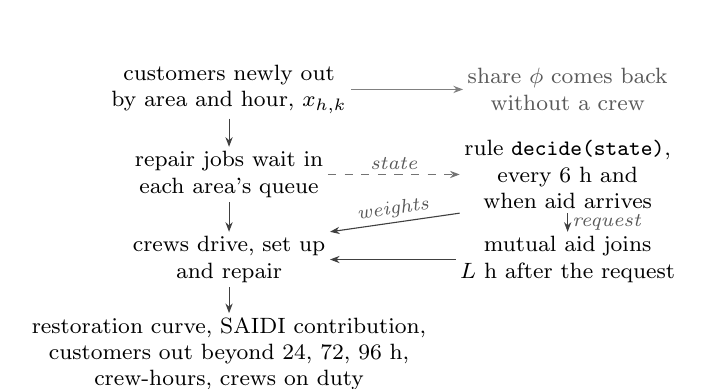
\begin{tikzpicture}[font=\footnotesize, >={Stealth[length=3.5pt]},
  lab/.style={align=center, inner sep=1.5pt}, line/.style={->, draw=black!75, line width=0.4pt},
  tag/.style={font=\scriptsize\itshape, text=black!65, inner sep=1.5pt}]
\node[lab] (dmg) at (0,0) {customers newly out\\by area and hour, $x_{h,k}$};
\node[lab] (jobs) at (0,-1.08) {repair jobs wait in\\each area's queue};
\node[lab] (crews) at (0,-2.16) {crews drive, set up\\and repair};
\node[lab] (out) at (0,-3.36) {restoration curve, SAIDI contribution,\\customers out beyond 24, 72, 96 h,\\crew-hours, crews on duty};
\node[lab, text=black!65] (auto) at (4.3,0) {share $\phi$ comes back\\without a crew};
\node[lab] (rule) at (4.3,-1.08) {rule \texttt{decide(state)},\\every \decisionH{} h and\\when aid arrives};
\node[lab] (aid) at (4.3,-2.16) {mutual aid joins\\$L$ h after the request};
\draw[line] (dmg) -- (jobs);
\draw[line] (jobs) -- (crews);
\draw[line] (crews) -- (out);
\draw[line, draw=black!50] (dmg.east) -- (auto.west);
\draw[line, dashed, draw=black!55] (jobs.east) -- node[tag, above] {state} (rule.west);
\draw[line] (rule.south west) -- node[tag, above, sloped] {weights} (crews.north east);
\draw[line] (rule.south) -- node[tag, right] {request} (aid.north);
\draw[line] (aid.west) -- (crews.east);
\end{tikzpicture}
\caption{The restoration loop. Damage replayed from the outage records becomes jobs, a rule decides where crews go
and when to ask for aid, and the engine reports reliability outcomes.}
\label{fig:engine}
\end{figure}

\subsection{What a rule sees and returns}

At each decision point, every \decisionH{} hours and when aid arrives, a rule receives the state of
Table~\ref{tab:state}. It returns non-negative weights $w_k$, one per area, and optionally an aid multiplier. No field
is normalized: all are in customers, crews, hours or km, and a rule that wants shares divides by customers served or
by crews itself. The engine turns the weights into targets $T_k=N(t)\,w_k/\sum_iw_i$, with $N(t)$ the crews on duty.
A crew freed in an area stays while the area is below its target. Otherwise it moves to the area with the largest
deficit in crews or, with proportional dispatch, the largest deficit relative to its target. A rule may also set the
job order and the dispatch mode. The default rule, current practice, weighs areas by their customers out.

\begin{table}[t]
\caption{The state a rule receives, per area unless noted}
\label{tab:state}
\centering\scriptsize
\setlength{\tabcolsep}{3pt}
\begin{tabular}{@{}llp{0.52\columnwidth}@{}}
\toprule
Field & Unit & Meaning \\
\midrule
\texttt{t} & h & time since the storm window began (scalar) \\
\texttt{out} & customers & out, waiting for a crew or under repair \\
\texttt{waiting\_jobs} & jobs & repair jobs in the queue \\
\texttt{working} & crews & working or driving to a job \\
\texttt{wait\_h} & h & wait of the oldest queued job \\
\texttt{arrived}, \texttt{restored} & customers & outages so far; restored by crews so far \\
\texttt{crews}, \texttt{aid\_crews} & crews & on duty with aid; brought by the request (scalars) \\
\texttt{forecast} & customers & interruptions the damage model expects \\
\texttt{customers} & customers & customers served \\
\texttt{dist\_km} & km & distances between area centroids (matrix) \\
\texttt{counties} & table & name, state, centroid, customer density \\
\midrule
\multicolumn{3}{@{}p{\columnwidth}@{}}{Returns: weights $w_k\ge0$, one per area, and an aid multiplier $m\ge0$ (only the first request counts)} \\
\bottomrule
\end{tabular}
\end{table}

\subsection{Outputs in reliability terms}

Every run returns the restoration curve and, from the outage $d_j$ of each job $j$ with $c_j$ customers, the
customer-hours $\sum_jc_jd_j$. Divided by the customers served and expressed in minutes, they give the storm's
contribution to SAIDI as defined in IEEE Std 1366, with major event days included \cite{ieee1366}. Divided by the
customers interrupted they give the event's CAIDI. A run also counts customers out beyond 24, 72 and 96 hours and
reports the time to restore the last customer, the worst area's mean outage, paid crew-hours (local crews from the
start of the storm and aid crews from the request, both to the end of restoration), crew-hours on jobs and on the road,
and the crews on duty once aid has joined.

\subsection{Interfaces}

StormCrews runs from Python, from a command line and from YAML scenario files, and an interactive notebook lets a
user without code pick a storm, move the what-if and crew settings and compare the run with a pinned baseline. The repository documents every interface, scenario key and metric.

\section{What It Is For and What It Is Not For}\label{sec:use}

StormCrews answers regional questions on real storms (Table~\ref{tab:use}), and its simplifications set the limits.
One pooled fleet serves a whole region, while utilities restore their own territories, so the split of outages
between utilities is not reproduced. Crews drive between area centroids. There is no feeder topology, no switching
and no power flow. The damage of a real storm is replayed, not generated, except through the what-if model, which is
associational. Rules that request aid early read the hour of the peak from the data.

\begin{table}[t]
\caption{Questions StormCrews can and cannot answer}
\label{tab:use}
\centering\scriptsize
\setlength{\tabcolsep}{3pt}
\begin{tabular}{@{}p{0.47\columnwidth}p{0.47\columnwidth}@{}}
\toprule
Fit for & Not fit for \\
\midrule
How the SAIDI contribution and long outages of past storms respond to fleet size, aid lag and restoration rules &
Dispatching or routing one utility's crews in a live storm \\
Weather what-ifs on real storms (stronger gusts, wetter soil) at regional scale &
Switching sequences, feeder reconfiguration, power flow, voltage or protection \\
Comparing rules on a common, reproducible set of storms (researchers, regulators) &
Estimated times of restoration for customers or feeders \\
Checking restoration standards and long-outage counts a regulator may set &
Outcomes inside an area or split by utility territory \\
\bottomrule
\end{tabular}
\end{table}

\section{Calibration and Validation}\label{sec:val}

Each storm has three parameters, the local fleet $N_0$, the mean repair time $\bar R$ and the job-size dispersion
$\sigma$. In the anchored calibration used here, $N_0$ is set so that the local fleet plus the usual aid equals
\anchorRatio{} crews per 1,000 customers out at the observed peak. That is the median of \nAnchors{}
public filings from New England and Pennsylvania that report line crews at work together with the same
utility's peak (\anchorMin{} to \anchorMax{} per 1,000; the Pennsylvania report counts line workers, taken at two per
crew \cite{papuc2025storm}). The median fleet is \fleetNE{} crews in New England and \fleetPA{} in Pennsylvania
and West Virginia. $\bar R$ is then fitted so that current practice reproduces the observed customer-hours, and
$\sigma$ so that the curve matches the hours from the peak to one half and one tenth of it. Customer-hours and the two
decay times are therefore targets. The peak is not, so it checks the fit, and it runs low under every calibration
(\peakAllMin{} to \peakAllMax{} of the observed, median over storms).

Because that fit is in sample, every storm was also predicted with parameters from the others. Leaving each storm out,
$\log\bar R$ is regressed on the log of the peak customers out over the other storms of its region and $\sigma$ is
their median, while the fleet keeps the anchor. Table~\ref{tab:val} and Fig.~\ref{fig:val} compare the two. Out of
sample, a storm's customer-hours miss by \chErrOutNE\,\% in New England and \chErrOutPA\,\% in Pennsylvania and West
Virginia at the median, and fall within 25\,\% for \chWithinOutNE\,\% and \chWithinOutPA\,\% of the storms. The hours
from the peak to a tenth of it miss by \tNinetyOutNE{} and \tNinetyOutPA{} hours at the median. Summed over each
region, held-out customer-hours come to \chPooledOutNE{} and \chPooledOutPA{} of those observed. The simulator replays
observed storms closely and predicts an unseen storm only roughly.

The county pattern shows what pooling crews leaves out. In Isaias, Connecticut lost \isaiasCHObsCT{} customer-hours per customer
and the rest of New England \isaiasCHObsRest. The simulation gives \isaiasCHSimCT{} and \isaiasCHSimRest{}
(Fig.~\ref{fig:maps}): it puts the outages in the right places but spreads the long ones more evenly than the
utilities, each restoring its own territory, did.


\begin{table}[t]
\caption{Current practice against every observed storm, anchored calibration, seed 0}
\label{tab:val}
\centering\scriptsize
\setlength{\tabcolsep}{2.6pt}
\begin{tabular}{@{}llrrrrrr@{}}
\toprule
Region & Parameters & \multicolumn{3}{c}{Customer-hours (targeted)} & Peak & \multicolumn{2}{c}{Decay error (h)} \\
\cmidrule(lr){3-5}\cmidrule(lr){7-8}
 & & sim/obs & error & within & sim/obs & to 50\,\% & to 10\,\% \\
 & & median & median & 25\,\% & median & median & median \\
\midrule
NE (\nStormsNE) & own storm & \chRatioInNE & \chErrInNE\,\% & \chWithinInNE\,\% & \peakRatioInNE & \tFiftyInNE & \tNinetyInNE \\
NE (\nStormsNE) & held out & \chRatioOutNE & \chErrOutNE\,\% & \chWithinOutNE\,\% & \peakRatioOutNE & \tFiftyOutNE & \tNinetyOutNE \\
PA--WV (\nStormsPA) & own storm & \chRatioInPA & \chErrInPA\,\% & \chWithinInPA\,\% & \peakRatioInPA & \tFiftyInPA & \tNinetyInPA \\
PA--WV (\nStormsPA) & held out & \chRatioOutPA & \chErrOutPA\,\% & \chWithinOutPA\,\% & \peakRatioOutPA & \tFiftyOutPA & \tNinetyOutPA \\
\bottomrule
\end{tabular}
\end{table}

\begin{figure*}[t]
\centering
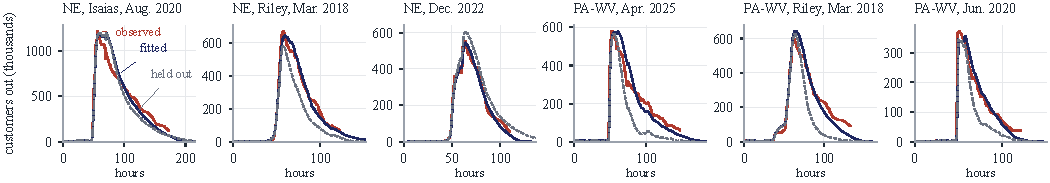
\includegraphics[width=\textwidth]{figures/validation.pdf}
\caption{The fitted simulator follows observed restoration, and parameters borrowed from other storms follow it less
closely. Observed EAGLE-I customers out (red), current practice with the storm's own anchored parameters (navy) and
with repair time and dispersion predicted from the other storms of its region (gray, dashed); six storms, seed 0.}
\label{fig:val}
\end{figure*}

\begin{figure*}[t]
\centering
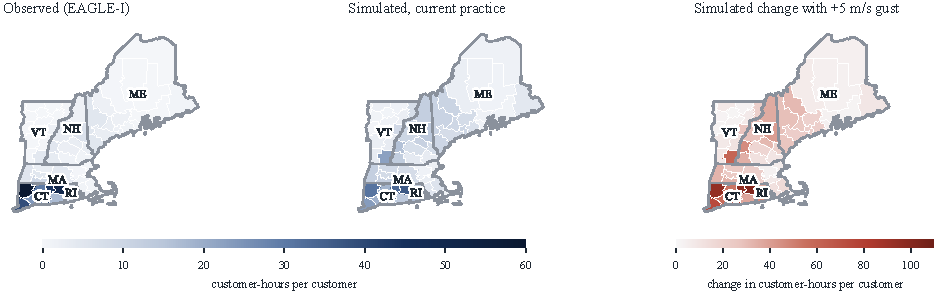
\includegraphics[width=\textwidth]{figures/isaias_maps.pdf}
\caption{The simulator places a real storm's outages where they happened. Tropical Storm Isaias by county: observed
customer-hours per customer (EAGLE-I), the same simulated under current practice with the anchored calibration (seed
1), and the simulated change if peak gusts had been 5\,m/s stronger.}
\label{fig:maps}
\end{figure*}

\section{Illustrations}\label{sec:demo}

Each illustration below is one command. It runs current practice on the \nStormsNE{} New England storms with the
anchored calibration and \nSeeds{} seeds. Summed over those storms, the simulated SAIDI contribution is \saidiNE{}
minutes, and \overSeventyTwoNE{} thousand customers stay out beyond 72 hours.

\emph{Weather.} Raising the peak gust by 5\,m/s in every county, through the damage model, multiplies the customers
interrupted by \gustInterX{}, the SAIDI contribution by \gustSaidiX{} and the customers out beyond 96 hours by
\gustOverNinetySixX{} (Fig.~\ref{fig:demos}a). The same crews face a longer queue. The median storm takes
\gustEndFive{} hours to restore instead of \gustEndZero{}, and paid crew-hours grow \gustPaidCHAbs\,\%.

\emph{Crew resources.} Across the range the filings report, \anchorMin{} to \anchorMax{} crews per 1,000 customers out
at the peak, the SAIDI contribution goes from \crewsMinSaidiAbs\,\% above to \crewsMaxSaidiAbs\,\% below its anchored
value (Fig.~\ref{fig:demos}b). Returns diminish. Going from \anchorRatio{} to \anchorMax{} crews per 1,000 cuts SAIDI
by \crewsMaxSaidiAbs\,\% and the customers out beyond 72 hours by \crewsMaxOverSeventyTwoAbs\,\%, but it takes
\crewsMaxPaidAbs\,\% more paid crew-hours and \crewsMaxTravelAbs\,\% more driving. Aid that arrives 12 hours after the
request instead of \aidLeadH{} changes SAIDI by \lagTwelveSaidi\,\%, and a 48-hour lag by \lagFortyEightSaidi\,\%
(Fig.~\ref{fig:demos}c).

\emph{Restoration rules.} Table~\ref{tab:rules} compares job orders and dispatch modes. Serving the oldest job first
instead of the largest raises SAIDI by \ruOldSaidiRelAbs\,\% and lengthens the tail too, because large faults wait
behind small ones, even though crews drive \ruOldTravelRelAbs\,\% less. Proportional dispatch leaves SAIDI almost
unchanged (\ruProSaidiRel\,\%) and shortens the worst county's mean outage by \ruProWorstRelAbs\,\%. A crew freed in a
busy area then goes to the area furthest behind its own target rather than the one short of most crews.

\begin{figure*}[t]
\centering
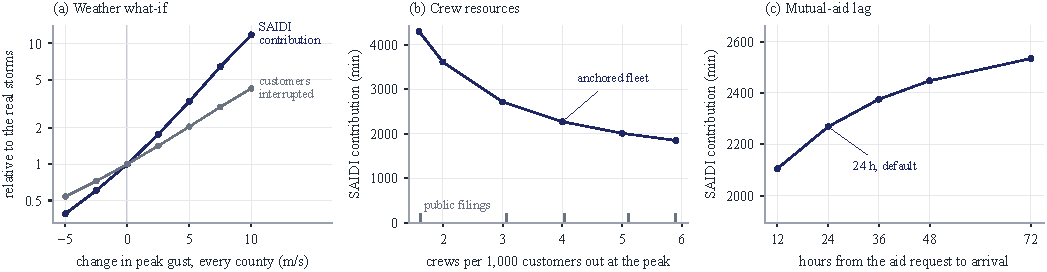
\includegraphics[width=\textwidth]{figures/demos.pdf}
\caption{Stronger gusts add outage minutes faster than interruptions, and more crews help with diminishing returns.
Simulated current practice on the \nStormsNE{} New England storms, anchored calibration, mean of \nSeeds{} seeds.
(a) Peak gust changed in every county. (b) Local fleet from \anchorMin{} to \anchorMax{} crews per 1,000 customers
out at the peak, the range of the public filings (ticks). (c) Hours from the aid request to arrival.}
\label{fig:demos}
\end{figure*}

\begin{table}[t]
\caption{Restoration rules, \nStormsNE{} New England storms, sums over storms}
\label{tab:rules}
\centering\scriptsize
\setlength{\tabcolsep}{2.6pt}
\begin{tabular}{@{}lrrrrrr@{}}
\toprule
Rule & SAIDI & \multicolumn{3}{c}{Customers out beyond} & Worst & Travel \\
\cmidrule(lr){3-5}
 & (min) & 24 h (M) & 72 h (k) & 96 h (k) & area (h) & (k crew-h) \\
\midrule
Largest first & \ruLarSaidi & \ruLarOverTwentyFour & \ruLarOverSeventyTwo & \ruLarOverNinetySix & \ruLarWorst & \ruLarTravel \\
Oldest first & \ruOldSaidi & \ruOldOverTwentyFour & \ruOldOverSeventyTwo & \ruOldOverNinetySix & \ruOldWorst & \ruOldTravel \\
Proportional dispatch & \ruProSaidi & \ruProOverTwentyFour & \ruProOverSeventyTwo & \ruProOverNinetySix & \ruProWorst & \ruProTravel \\
\bottomrule
\end{tabular}
\vspace{1pt}

\raggedright\scriptsize Worst area: mean outage of the worst county, averaged over storms. Mean of \nSeeds{} seeds.
\end{table}

\emph{Assumptions.} The figure of \custPerJob{} customers per job is an assumption. It lies between the mean of
about 31 customers per outage at the peak of the five storms in \cite{walsh2018abm} and the median of about 38 over
55 Connecticut storms read from Fig.~4 of \cite{wanik2018etr}. Table~\ref{tab:perjob} refits $\bar R$ at \pjLow{} and \pjHigh{} customers per job and reruns the
illustrations. The relative effects move by a few points, while the long-tail counts and crew-hours change much more,
so those depend on the assumption. Moving the reactive trigger from 0.5\,\% to 2\,\% of customers out changes SAIDI
by \trigLowSaidi\,\% and \trigHighSaidi\,\%.

\begin{table}[t]
\caption{Sensitivity to the customers behind one repair job}
\label{tab:perjob}
\centering\scriptsize
\setlength{\tabcolsep}{2.4pt}
\begin{tabular}{@{}rrrrrrr@{}}
\toprule
Customers & Refitted & \multicolumn{3}{c}{SAIDI change against the real storms} & Out $>$96 h & On jobs \\
\cmidrule(lr){3-5}
per job & $\bar R$ (h) & gust $+5$ & 75\,\% fleet & 48 h aid lag & (k) & (M crew-h) \\
\midrule
\pjLow & \pjLowRepair & $\times$\pjLowGust & \pjLowFleet\,\% & \pjLowLag\,\% & \pjLowOverNinetySix & \pjLowBusy \\
\pjMid & \pjMidRepair & $\times$\pjMidGust & \pjMidFleet\,\% & \pjMidLag\,\% & \pjMidOverNinetySix & \pjMidBusy \\
\pjHigh & \pjHighRepair & $\times$\pjHighGust & \pjHighFleet\,\% & \pjHighLag\,\% & \pjHighOverNinetySix & \pjHighBusy \\
\bottomrule
\end{tabular}
\end{table}


\section{Contribution Against Existing Tools}\label{sec:related}

Table~\ref{tab:related} compares StormCrews with the closest tools. Walsh et al. model Connecticut crews and
mutual-aid crews on five storms with a utility's data \cite{walsh2018abm}. Oak Ridge's RePOWERD work routes crews over
damaged roads on hypothetical outages \cite{kar2022repowrd,chen2023multiagent}, and Willems et al. estimate the
restoration times of five hurricanes statistically \cite{willems2024probabilistic}. Open platforms are reproducible
but do not replay storms with crews and aid. InfraRisk sends repair crews over the road network of test cities
\cite{balakrishnan2022infrarisk}, PowerModelsRestoration orders restoration by optimization
\cite{rhodes2021powermodelsrestoration} and GridLAB-D simulates feeders \cite{chassin2014gridlabd}. The EAGLE-I
outage records give real storms without decisions \cite{brelsford2024eaglei}. StormCrews brings these pieces together:
real storms calibrated from public records, crews with travel, mutual aid with its lag, rules a user writes, and
results in reliability indices, all open and checked by \nTests{} tests.

\begin{table}[t]
\caption{StormCrews and related tools ($\bullet$ yes, $\circ$ partly, -- no)}
\label{tab:related}
\centering\scriptsize
\setlength{\tabcolsep}{2.2pt}
\begin{tabular}{@{}lccccc@{}}
\toprule
Tool & Real & Public & Crews, & Mutual & Open, \\
 & storms & data & travel & aid & reproducible \\
\midrule
\textbf{StormCrews} & $\bullet$ & $\bullet$ & $\bullet$ & $\bullet$ & $\bullet$ \\
Walsh et al. \cite{walsh2018abm} & $\bullet$ & -- & $\bullet$ & $\bullet$ & $\circ$ \\
RePOWERD \cite{kar2022repowrd,chen2023multiagent} & $\circ$ & $\circ$ & $\bullet$ & $\circ$ & -- \\
Willems et al. \cite{willems2024probabilistic} & $\bullet$ & $\bullet$ & -- & -- & -- \\
InfraRisk \cite{balakrishnan2022infrarisk} & -- & $\bullet$ & $\bullet$ & -- & $\bullet$ \\
PowerModelsRestoration \cite{rhodes2021powermodelsrestoration} & -- & $\bullet$ & -- & -- & $\bullet$ \\
GridLAB-D \cite{chassin2014gridlabd} & -- & $\bullet$ & -- & -- & $\bullet$ \\
EAGLE-I outage data \cite{brelsford2024eaglei} & $\bullet$ & $\circ$ & -- & -- & $\bullet$ \\
\bottomrule
\end{tabular}
\end{table}

\section{Availability}\label{sec:avail}

The code and data are at \url{https://github.com/abrahambohorquez/stormcrews} (version \version, Python 3.10 or
later). It installs with pip from GitHub, or from a clone with \mbox{\texttt{pip install -e .}} run in its folder. A run takes a scenario, a
storm, a rule and a seed, and each result reported here comes from one command:\\[2pt]
\noindent\begin{minipage}{\columnwidth}
\begin{Verbatim}[fontsize=\scriptsize,frame=single,framesep=1mm]
pip install \
  git+https://github.com/abrahambohorquez/stormcrews

from stormcrews import Simulator
from stormcrews.rules import CurrentPractice
sim = Simulator("new_england", calibration="anchored")
r = sim.run(CurrentPractice(), storm="isaias", seed=1)
print(r.metrics["saidi_min"], r.metrics["over_72h"])

python paper_gtdla/experiments.py all
python paper_gtdla/make_figures.py   # every figure
python paper_gtdla/make_macros.py    # every number
\end{Verbatim}
\end{minipage}\vspace{5pt}

\noindent
The code is under the MIT license and the derived data under CC~BY~4.0, with the attributions of the repository's
data license. The outage data are from EAGLE-I, Oak Ridge National Laboratory, under CC~BY~4.0 \cite{eaglei2026data}.
The weather contains modified Copernicus Climate Change Service information, retrieved through Open-Meteo
(weather data by Open-Meteo.com) under CC~BY~4.0 \cite{c3s2018era5,zippenfenig2024openmeteo}. Neither Oak Ridge
National Laboratory, the U.S. Department of Energy nor ECMWF endorses StormCrews.

\section{Conclusion}

StormCrews turns public outage records into a restoration simulator that a distribution planner, a regulator or a
researcher can rerun and change. On \nStorms{} real storms it shows what a rule, a fleet size or a stronger storm does
to the SAIDI contribution, to the customers out for days and to the crew-hours spent. It replays observed storms
closely and predicts unseen ones roughly. It pools each region's crews, so it serves regional what-ifs and the
comparison of rules, not the dispatch of one utility. Utility service territories and a third region come next.

\bibliographystyle{IEEEtran}
\bibliography{refs}

\end{document}
